\section{From the Books of Valens Concerning the Numerical Lot and the Length of Life. The Same Author on the Topic of Propitious Times, with Examples (10K,7P)}
\index{\textit{Petosiris}}
\index{lots!Life}
\index{length of life}
There is another numerical method, which \mn{Petosiris} King Petosiris has mystically explained, suitable for determining the length of life and the propitious and impropitious times. As a result, whenever we find the controller or the houseruler <configured> appropriately, we will use the method described above for the allotment. If we do not find them to be such, we will use the following method.

It will be necessary to determine if the nativity happened at new or full moon. If it happened at new moon, determine the number of degrees from \textbf{/146K/} the new moon to the position of the \Moon\, at the delivery itself, then count this distance from the Ascendant in the order of the signs. The ruler of the term where the count stops will be the houseruler of Life and of the vital sector. 

If the nativity is at full moon, it will be necessary to determine the degrees from the \Moon’s position at the delivery to its position at the next new moon. Then count this distance from the Ascendant, not in the order of the signs, but in the direction of diurnal motion (towards MC). The ruler of the term where the count stops will be considered the houseruler. It will be necessary to examine it and the sign where the count stopped to see which <luminary> is more closely related to it, the \Sun\, for masculine <signs>,or the \Moon\, for feminine <signs>.

If the sign where the count stopped happens to be related to the \Sun\xspace when the \Sun\xspace has control, and if the
ruler of the term is also in harmony with the \Sun\xspace and happens to be favorably configured with the \Sun, then
it will allot the maximum number of years. 

If this sign is found to be related (i.e. male, as would be appropriate for the \Sun), and if the ruler of the term is opposite the \Sun, precedes the Ascendant, or is in ecliptic places\footnote{Probably being conjunct the \Moon's nodes, which is where eclipses occur.}, then it will become the anaereta of the chronocratorship, or it will allot the minimum number of years. (The masculine signs belong to the \Sun; the feminine to the \Moon.) Consequently it will be necessary to examine how the ruler of the term is configured with respect to the controller and with respect to the ruler of the sign. If it is found to be in its own sign or in operative signs, the length of life will reach its maximum. If it is found to be favorably configured with respect to one, but unsuitably configured with respect to the other, it will allot the mean number of years. 

\index{configuration!unsuitable}
If the houseruler of the sign where the count stopped is unsuitably configured with respect to the controller and the \textbf{/139P/} operative sign, being either turned away or in <the XII Place of the> Bad Daimon, then the nativity will lack a houseruler. In such a case it will again be necessary to examine the control of the \Sun\, and \Moon. 

If the rulers of the term and of the sign are configured well and harmoniously with the \Sun\xspace and \Moon, then the vital sector will be considered as starting at the degree of the term.

Generally speaking, in this method it will be necessary to examine the houseruler with reference to the influences of the angles, as was demonstrated for the \textsl{horimaea}\footnote{Schmidt spells this as \textsl{h\=orimaia} and says this refers to a method not described by Valens (at least under this name) but described in Book 3 of [Ptolemy's] \textsl{Tetrabiblios} ``where it refers to a special case where the apheta is in the 7th or 9th places and is directed against the order of the signs instead of with the order of the signs'' (VRS3 footnote p55); however, it may be related to the general rules given earlier for determining the condition of rank, prosperity, and happiness.}: it may be rising, setting, at an angle, not at an angle; it may switch positions with the ruler of its sign\footnote{i.e. be in mutual reception by sign or exaltation.} or be inharmonious with it. Use these facts to make your judgement. 

\index{twins}
Likewise <it will be necessary to> look at the rays of the anaeretic stars and to check if the vital sector starts at the beginning of the terms or at the end. It is necessary to consider all of this \textbf{/147K/} in order to calculate short- or long-lived nativities—or even the nativities of twins, because often if a malefic term rules the vital sector or if the houseruler is unfavorably situated, the first-born
becomes short-lived, but the next-born, if the term or the houseruler changes, becomes long-lived and a foundation for his existence arises. Consequently, a change of one or two degrees often has a very great effect.

An example: \Sun\xspace in \Taurus\xspace 25° 18', \Moon\xspace in \Aquarius\xspace 7° 10', \Saturn\xspace in \Aries\xspace 24°, \Jupiter\xspace in \Taurus\xspace 4° 25', \Mars\xspace in \Cancer\xspace 22° 53', \Venus\xspace in \Gemini\xspace 28° 16', \Mercury\xspace in \Gemini\xspace 6°, Ascendant in \Capricorn\xspace 27°
\footnote{\textit{Greek Horoscopes} dates the chart (L114,V) to approximately March 13, 114 AD about 10 p.m. (p.110)}. 

\clearpage
\begin{wrapfigure}[15]{R}{7cm}
\centering
\vspace{-20pt}
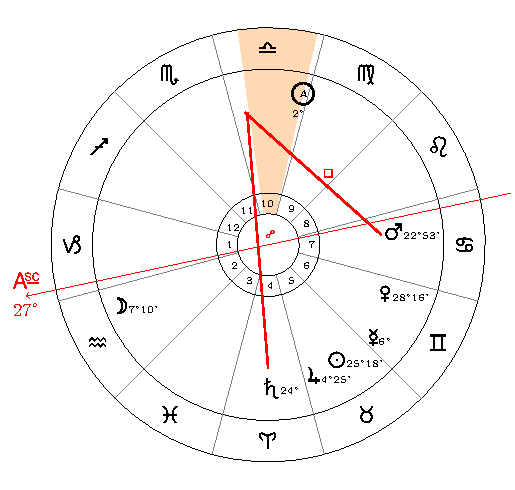
\includegraphics[width=0.68\textwidth]{charts/3_10_1}
\caption{Chart 44 [III.10.1, GH L114]}
\label{fig:chart44}
\end{wrapfigure} 

Since this was a full-moon nativity, I took the distance from the \Moon’s position <at birth> to the next new moon, which was at \Gemini\xspace 2° 25'. The distance is 115°. I subtract this from the Ascendant and stop at \Libra\xspace 2°. The vital sector stretches from this point\footnote{At 2\Libra, where the lot is. Robert Hand calls it the \textsl{Lot of Aphesis} (VRS3 p56).} to the radiation of the malefics. \Saturn\xspace casts its rays from a point in opposition and \Mars\xspace from a point square with the same degrees <in \Libra> and cause death. \Jupiter\xspace was turned away\footnote{\Jupiter\, is in the 8th place from \Libra\, and so \textsl{averse} or ``turned away''.}; \Venus\,\footnote{ \Venus\, (the benefic of the sect) is in the 6th, an unfavourable house, and throws her trine to 28\Libra, outside the vital sector.} was unfavorably situated and unable to help. The native lived 28 years 9 months\footnote{Robert Hand calculates this using 40° for \Libra's ascenional times and the difference between \Mars's square at 22 \Libra: 22/30 x 40 = 29.33 $\approx$ 29 years 4 months, close to Valens 28 years 9 months (VRS3 p56). }.

\newpage
\textbf{/140P/} Another example: \Sun\xspace in \Sagittarius\xspace 12° 16', \Moon\xspace in \Sagittarius\xspace 17° 24', \Saturn\xspace in \Libra\xspace 11° 33', \Jupiter\xspace in \Gemini\xspace 19° 11;, \Mars\xspace in \Scorpio\xspace 4° 20', \Venus\xspace in \Libra\xspace 26°, \Mercury\xspace in \Scorpio\xspace 27°,
Ascendant in \Libra\xspace 20°
\footnote{\textit{Greek Horoscopes} dates the chart (L127,XI) to approximately Nov. 23, 127 AD about 3 a.m. (p.110)}.

\clearpage
\begin{wrapfigure}[15]{R}{7cm}
\centering
\vspace{-20pt}
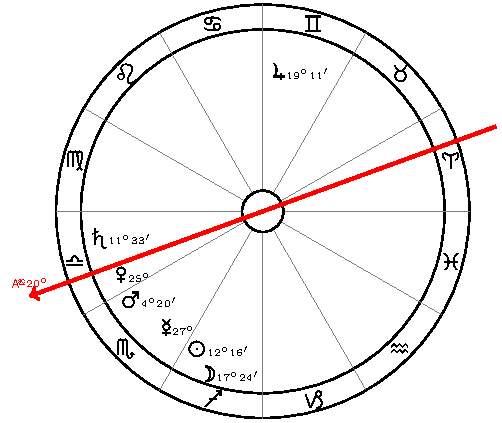
\includegraphics[width=0.68\textwidth]{charts/3_10_2}
\caption{Chart 45 [III.10.2, GH L127]}
\label{fig:chart45}
\end{wrapfigure} 


I take the distance from the degree of the new moon to the \Moon’s position <at birth>; this is 5°. I count this from the Ascendant and stop at \Libra\xspace 25°. The vital sector stretched from there\footnote{25\Libra\, would be the position of the Lot of Aphesis.} to the position of \Mars, \Scorpio\xspace 5°. The native died in his twelfth year\footnote{Robert Hand calculates the 12 years as coming from the ascensional times of \Libra\, (40) and \Scorpio\, (36) such that 5° of \Libra\, (5/30 x 40) plus 5° degrees of \Scorpio\, (5/30 x 36) = 6°40' + 6° = 12°40' (VRS3 p57).}. If this encounter <with \Mars> had not happened, he would have lived the years of \Venus, 84\footnote{\Venus's greater years, which are usually given to be 82, not 84.}.

\newpage